\chapter{Аналитическая часть}

В аналитической части проведён анализ предметной области онлайн-версии
настольной игры <<Эпичные схватки боевых магов: Крутагидон>>, в том числе
описание типов карт, механики работы рынка и условий победы. Сформулированы
требования и ограничения к приложению, формализованы данные и роли
пользователей.

\section{Описание предметной области}

Онлайн-версия упомянутой колодостроительной (deck-building) игры представляет
собой многопользовательскую карточную игру, в которой игроки сражаются между
собой, используя карты из общей системы карт. Для реализации используются
механики, описанные в правилах игры, но некоторые объекты
переименованы~\cite{rules}.

Игровой процесс строится на последовательности ходов \textit{игроков} ---
участников игровой сессии, обладающих параметрами состояния (например,
здоровье, очки крутости) и взаимодействующих с игровыми объектами в процессе
игры. Во время своего хода игрок может разыгрывать карты из своей руки,
получать игровой ресурс --- \textit{эхо} --- и использовать его для покупки
новых карт из рынка. Купленные карты добавляются в личную колоду игрока и могут
быть использованы в дальнейшем. В конце каждого хода все карты, с которыми
игрок начинал свой ход, сбрасываются, а на руку набираются новые~\cite{rules}.

Игрок обладает личной колодой карт, которая используется в процессе игры.
Колода формируется из стартовых карт (началок), а затем пополняется новыми
картами, приобретёнными игроком на рынке. Механика работы рынка приведена ниже.
В ходе игры карты могут находиться в различных состояниях (колодах): рука,
добор, стол, сброс, рынок, основная колода и игровой сброс~\cite{rules}.

Типы колод:
\begin{itemize}
	\item рука (hand) --- просматриваемые и разыгрываемые карты, с которыми
	      игрок начинает ход;
	\item колода добора (draw) --- колода игрока, из которой формируется
	      рука и осуществляется добор карт;
	\item стол (table) --- карты, которые игрок разыграл на текущем ходу,
	      доступны к просмотру всем игрокам;
	\item сброс (discard) --- колода для сброшенных карт, формирует колоду
	      добора, когда в ней заканчиваются карты;
	\item рынок (market) --- колода из 5 открытых карт, которые доступны
	      для просмотра всем игроками и покупки игроку в свой ход;
	\item основная игровая колода (deck) --- колода, из которой формируется
	      рынок;
	\item сброс игры (banish) --- карты, которые сбрасываются без возврата
	      в игру.
\end{itemize}

В течение ходов игроки могут получать урон от атак других игроков или атаковать
самостоятельно, пополнять руку новыми картами, лечиться, набирать внутриигровую
валюту покупки карт --- эхо. Атаки уменьшают количество очков здоровья игрока
и, если здоровье игрока становится меньше или равно 0, то игрок на этом ходу
умирает, получает <<памятку о бренности бытия>>, отмечающую его смерть, и сразу
же восстанавливается со стандартным количеством очков здоровья~\cite{rules}.

Игра заканчивается, когда все выделенные на игру памятки о бренности бытия
заканчиваются. Победитель определяется подсчётом очков крутости, которые
складываются из очков крутости каждой карты, которой обладает игрок на момент
завершения игры~\cite{rules}.

Для корректной работы системы необходимо хранить информацию об игроках, текущих
партиях, составе колод игроков и колод игры, картах и типах карт.

\section{Типы карт}
Карты являются основным элементом для реализации игровой механики. Каждая карта
обладает определённым набором характеристик и эффектов и принадлежит
определенному типу.

В системе используются следующие типы карт: началка, существа (дварф, эльф,
дракон, волшебник), штуки и чертоги.
\begin{description}
	\item[Началка] --- карты стартовой колоды игроков.

	\item[Дварф, эльф, дракон, и волшебник] --- карты существ с
		определёнными характеристиками.

	\item[Штука] --- карты предметов с определёнными характеристиками.

	\item[Чертог] --- карты локаций, дающие постоянные эффекты.
\end{description}

Карты могут обладать следующими эффектами: защита, добор, атака, хилл, буст
руки и буст эхо.

\begin{description}
	\item[Защита] --- позволяет избежать атаки другого игрока.

	\item[Добор] --- позволяет взять и разыграть дополнительные карты.

	\item[Атака] --- позволяет атаковать другого игрока.

	\item[Хилка] --- позволяет восстановить часть здоровья.

	\item[Буст руки] --- позволяет разыгрывать больше карт, действует
		постоянно.

	\item[Буст эхо] --- увеличивает базовое значение ресурса эхо игрока,
		действует постоянно.
\end{description}

Каждая карта имеет следующие свойства:
\begin{itemize}
	\item название;
	\item тип карты;
	\item изображение;
	\item эффект карты и его описание;
	\item числовая характеристика эффекта;
	\item значение эхо;
	\item стоимость для покупки;
	\item количество очков крутости.
\end{itemize}

\section{Механика работы рынка карт}

В каждой партии формируется рынок карт, из которого игроки могут приобретать
новые карты. Рынок состоит из пяти открытых карт, доступных для покупки, и
закрытой колоды, из которой рынок обновляется в начале каждого
хода~\cite{rules}.

После розыгрыша своих карт игрок может купить любое количество открытых карт
рынка, на которое у него хватает накопленного эхо. После покупки карта
удаляется из рынка и добавляется в личную колоду игрока~\cite{rules}.

На покупку карт накладываются следующие ограничения:
\begin{itemize}
	\item нельзя купить карт больше, чем есть открытых карт на рынке;
	\item одну и ту же карту нельзя купить больше одного раза;
	\item нельзя купить карту, отсутствующую на открытом рынке.
\end{itemize}

Для покупки карт используется накапливаемое игроком в течение хода эхо. Каждая
разыгранная карта может как увеличить, так и уменьшить или не изменить текущее
значение эхо~\cite{rules}.

Значение эхо хранится для каждого игрока отдельно, накапливается в течение хода
и после него сбрасывается до нуля (или базового значения конкретного игрока,
если он использовал карты, меняющие этот показатель)~\cite{rules}.

При покупке карт с рынка текущее значение эхо уменьшается на стоимость
купленной карты. Карта может быть куплена только в том случае, когда текущее
значение эхо игрока не меньше стоимости карты~\cite{rules}.

\section{Категории пользователей}
В системе предусмотрено несколько категорий пользователей, обладающих разными
правами доступа:

\begin{description}
	\item[Неавторизованный пользователь (гость)] --- пользователь, который
		может просматривать правила игры и каталог карт.

	\item[Авторизованный пользователь] --- пользователь, который может
		делать
		то же самое, что и неавторизованный, а также может создавать
		игры или
		присоединяться к уже созданным.

	\item[Игрок] --- пользователь, находящийся в игровой партии, способный
		выполнять ходы.

	\item[Модератор] --- пользователь, обладающий всеми возможностями
		авторизованного пользователя, который может блокировать и
		разблокировать других
		пользователей, просматривать текущие игры, временно их
		останавливать или
		завершать.

	\item[Мастер] --- пользователь, который может делать всё то же, что и
		модератор, а также добавлять новые карты, менять или удалять
		уже существующие.
\end{description}

Диаграмма вариантов использования разрабатываемой системы представлена на
рисунке~\ref{img:r-use-case}.

\begin{figure}[H]
	\centering
	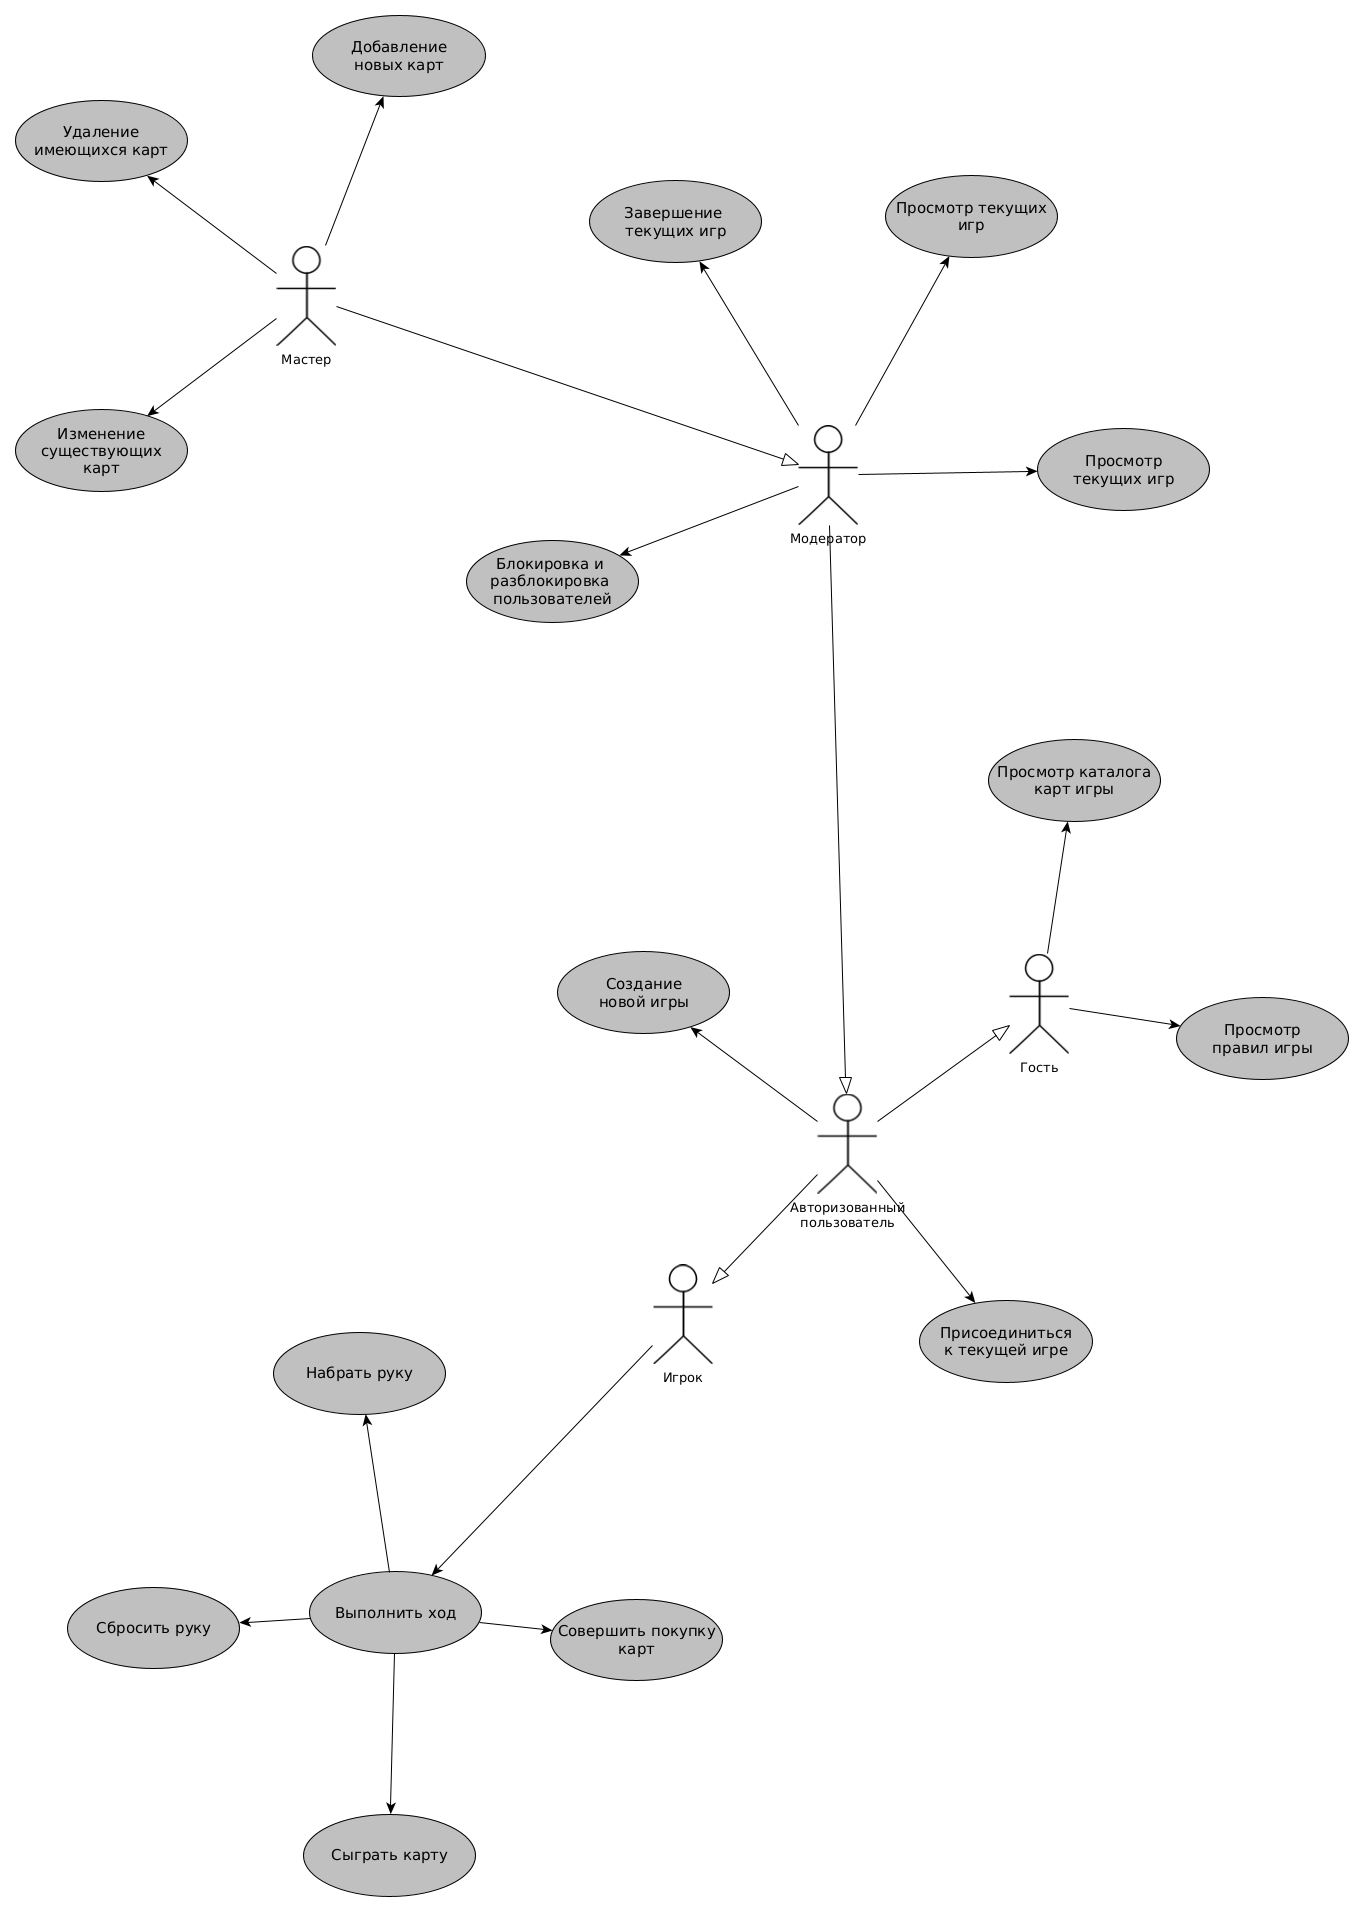
\includegraphics[width=1\linewidth]{../img/r-use-case}
	\caption{Диаграмма вариантов использования разрабатываемой системы}
	\label{img:r-use-case}
\end{figure}

\section{Требования к разрабатываемому приложению}
Разрабатываемый сайт предназначен для одного или нескольких гостей, способных
просматривать игровые карты и правила игры, и пользователей, способных
авторизоваться и быть участниками игровых партий.

Таким образом, разрабатываемое приложение должно обладать следующей
функциональностью:
\begin{enumerate}
	\item управление игровыми сессиями (создание, подключение и завершение
	      игры);
	\item взаимодействие игроков в рамках игровой сессии;
	\item отображение текущего состояния игры (поле, карты, колоды и прочие
	      игровые сущности);
	\item выполнение игровых действий пользователем (применение эффектов
	      карт,
	      покупка новых);
	\item обработка логики игры (подсчёт очков, применение правил, переходы
	      между состояниями);
	\item поддержка работы с колодами карт (формирование, перемешивание,
	      добор
	      и сброс карт);
\end{enumerate}

Таким образом, приложение должно обеспечивать полный цикл управления игровыми
сессиями, включая создание, участие в игре и просмотр результатов.

\section{Формализация данных}

В таблице~\ref{tbl:data} представлены сущности, используемые в базе данных.

\begin{longtable}{|>{\raggedright\arraybackslash}p{0.14\textwidth}|>{\raggedright\arraybackslash}p{0.14\textwidth}|>{\raggedright\arraybackslash}p{0.26\textwidth}|>{\raggedright\arraybackslash}p{0.12\textwidth}|>{\raggedright\arraybackslash}p{0.14\textwidth}|}
	\caption{Сущности и их свойства} \label{tbl:data}
	\\
	\hline
	\textbf{Сущность} & \textbf{Свойство} & \textbf{Метка}
	                  & \textbf{Тип}      &
	\textbf{Атрибут БД}
	\\
	\hline
	\endfirsthead
	\caption{Сущности и их свойства}
	\\
	\hline
	\textbf{Сущность} & \textbf{Свойство} & \textbf{Метка}
	                  & \textbf{Тип}      & \textbf{Атрибут БД}
	\\
	\hline
	\endhead
	\hline
	\endfoot
	\endlastfoot

	\textbf{Пользо-\newline ватель}
	                  & Псевдоним         & Имя пользователя, уникально
	                  & Строка            & \texttt{username}
	\\
	\cline{2-5}
	                  & Эл. почта         & Адрес почты, уникально
	                  & Строка            & \texttt{e-mail}
	\\
	\cline{2-5}
	                  & Пароль            & Хеш пароля
	                  & Строка            & \texttt{password}
	\\
	\cline{2-5}
	                  & Дата рег.         & Время создания аккаунта
	                  & DateTime          &
	\texttt{register\_\newline date}
	\\
	\hline

	\textbf{Игра}
	                  & Текущий ход       & Номер текущего хода
	                  & Целое число       &
	\texttt{current\_move}
	\\
	\cline{2-5}
	                  & Памятки           & Оставшееся кол-во памяток
	                  & Целое число       & \texttt{memos}
	\\
	\cline{2-5}
	                  & Время начала      & Момент старта партии
	                  & DateTime          & \texttt{time\_start}
	\\
	\cline{2-5}
	                  & Победитель        & Внешний ключ к Players, может
	быть NULL         & Целое число       &
	\texttt{winner}
	\\
	\hline

	\textbf{Игрок}
	                  & Пользователь      & Внешний ключ к Users
	                  & Целое число       & \texttt{user\_id}
	\\
	\cline{2-5}
	                  & Игра              & Внешний ключ к Games
	                  & Целое число       & \texttt{game\_id}
	\\
	\cline{2-5}
	                  & Здоровье          & Текущее здоровье
	                  & Целое число       & \texttt{health}
	\\
	\cline{2-5}
	                  & Лимит руки        & Макс. карт в руке
	                  & Целое число       & \texttt{hand\_limit}
	\\
	\cline{2-5}
	                  & Базовое эхо       & Базовый ресурс
	                  & Целое число       & \texttt{base\_echo}
	\\
	\cline{2-5}
	                  & Порядок хода      & Очередность хода игрока
	                  & Целое число       & \texttt{turn}
	\\
	\hline

	\textbf{Карта}
	                  & Название          & Название карты
	                  & Строка            & \texttt{title}
	\\
	\cline{2-5}
	                  & Эхо               & Количество эхо карты
	                  & Целое число       & \texttt{echo}
	\\
	\cline{2-5}
	                  & Стоимость         & Цена покупки
	                  & Целое число       & \texttt{cost}
	\\
	\cline{2-5}
	                  & Сила              & Значение эффекта
	                  & Целое число       & \texttt{power}
	\\
	\cline{2-5}
	                  & Тип карты         & Внешний ключ к Types
	                  & Целое число       & \texttt{card\_type}
	\\
	\cline{2-5}
	                  & Очки крутости     & Очки за карту
	                  & Целое число       & \texttt{cool\_points}
	\\
	\hline

	\textbf{Тип карты}
	                  & Действие          & Тип эффекта
	                  & Строка            & \texttt{action}
	\\
	\cline{2-5}
	                  & Постоянность      & Признак постоянного эффекта
	                  & Логический        &
	\texttt{if\_permanent}
	\\
	\hline

	\textbf{Колода}
	                  & Тип               & Тип (market, hand и т.д.)
	                  & Строка            & \texttt{type}
	\\
	\cline{2-5}
	                  & Открытость        & Могут карты быть просмотрены
	или нет           & Логический        &
	\texttt{if\_open}
	\\
	\cline{2-5}
	                  & Владелец          & Внешний ключ к Players, может
	быть NULL         & Целое число       &
	\texttt{owner\_id}
	\\
	\hline

	\textbf{Карта в колоде}
	                  & Колода            & Внешний ключ к Decks
	                  & Целое число       & \texttt{deck\_id}
	\\
	\cline{2-5}
	                  & Карта             & Внешний ключ к Cards
	                  & Целое число       & \texttt{card\_id}
	\\
	\cline{2-5}
	                  & Позиция           & Порядковый номер карты в
	стопке            & Целое число       &
	\texttt{position}
	\\
	\hline

	\textbf{Изображение}
	                  & Название          & Имя файла/заголовка
	                  & Строка            & \texttt{title}
	\\
	\cline{2-5}
	                  & Файл              & Путь к файлу изображения
	                  & Path              & \texttt{file}
	\\
	\hline
\end{longtable}

На рисунке~\ref{img:er} представлена диаграмма сущность-связь, отражающая
структуру базы данных и связи между сущностями.

\begin{figure}[H]
	\centering
	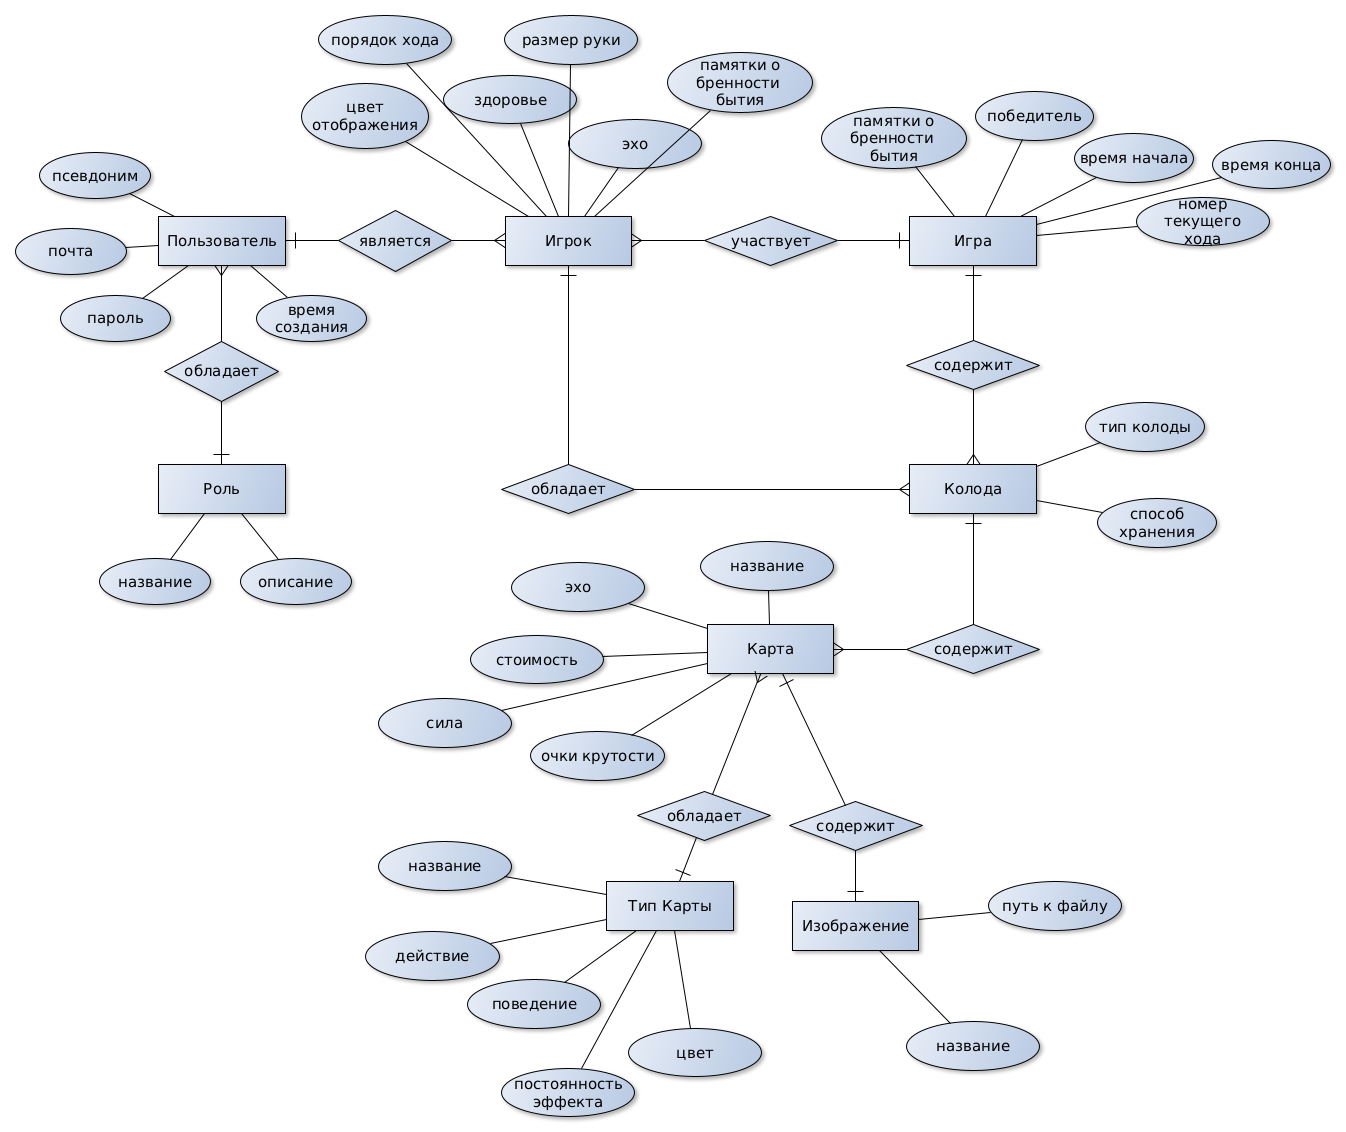
\includegraphics[width=1\linewidth]{../img/er.png}
	\caption{Диаграмма сущность-связь в нотации Чена}
	\label{img:er}
\end{figure}

\section{Выбор модели хранения данных}

В разрабатываемой системе предполагается хранение структурированных данных
предметной области, включающих сущности (например, пользователи, игровые
объекты, карты) и связи между ними. Для каждой сущности задан фиксированный
набор атрибутов и предусмотрены взаимосвязи, требующие поддержания целостности
и согласованности данных~\cite{lectures}.

Существует несколько основных моделей хранения данных:

\begin{description}
	\item[Дореляционная модель] --- данные хранятся в виде иерархических
		структур, файлов или сетевых баз данных. Эта модель не
		предполагает жёсткой
		схемы таблиц и характеризуется сложностью в обеспечении
		ссылочной целостности.
		Операции с данными требуют специализированного программного
		обеспечения, а
		структура данных тесно связана с применением. Дореляционный
		подход хорошо
		подходит для специализированных приложений, но неудобен для
		систем, требующих
		гибкости и универсальности~\cite{lectures}.

	\item[Реляционная модель] --- информация представляется в виде таблиц с
		явно определёнными атрибутами, первичными и внешними ключами,
		ограничениями
		целостности и уникальности. Реляционная модель обеспечивает
		строгое разделение
		структуры данных от логики приложения, позволяет использовать
		стандартный язык
		запросов (SQL), удобна для сложных операций и обеспечивает
		надёжность данных
		через механизмы транзакций~\cite{date}.

	\item[Постреляционная модель] --- Такие БД основаны на реляционных,
		однако
		отходят от их принципов в пользу более эффективного решения
		специфических
		задач. Одним из примеров таких особенностей выступает
		возможность вложенного
		хранения таблиц (хранения таблиц в таблицах), что невозможно в
		реляционных
		БД~\cite{postrel}.
\end{description}

С учётом требований разрабатываемой системы наиболее подходящей является
реляционная модель данных. Она позволяет явно определить структуру данных
(пользователи, игры, игроки, карты, колоды), обеспечить строгое соблюдение
ограничений целостности, поддержать сложные многотабличные запросы для анализа
состояния игры и гарантировать консистентность данных при одновременном доступе
нескольких игроков. Реляционная модель удобна для выполнения сложных запросов и
фильтрации информации.

\section*{Вывод}

В аналитической части была рассмотрена предметная область, были рассмотрены и
формализованы данные, подлежащие хранению и выбрана реляционная модель хранения
данных.